

\includegraphics[width=1.5cm]{images/pictograms/replication}

\includegraphics[height=1.25cm]{images/pictograms/FEM}

\lstinputlisting[language=bash,basicstyle=\small]{python_codes/fieldstone_143/keywords.key}

\begin{center}
Code at \url{https://github.com/cedrict/fieldstone/tree/master/python_codes/fieldstone_143}
\end{center}

\par\noindent\rule{\textwidth}{0.4pt}

%%%%%%%%%%%%%%%%%%%%%%%%%%%%%%%%%%%%%%%%%%%%%%%%%%%%%%%%%%%%%%%%%%%%%%%%%%%%%%%%%%%%%%%%%%%%%%%%%%%%

This \stone is based on \textcite{yahb13} (2013) published in Tectonics.
As for every \stone aiming at reproducing results off a publication I here include de abstract
of the article:

\begin{center}
\begin{minipage}{13cm}
{\small 
Passive margins often exhibit uplift, exhumation, and tectonic inversion. We speculate
that the compression in the lithosphere gradually increased during the Cenozoic, as seen in
the number of mountain belts found at active margins during that period. Less clear is how
that compression increase affects passive margins. In order to address this issue, we design a
2-D viscous numerical model wherein a lithospheric plate rests above a weaker mantle. It is
driven by a mantle conveyor belt, alternatively excited by a lateral downwelling on one side,
an upwelling on the other side, or both simultaneously. The lateral edges of the plate are
either free or fixed, representing the cases of free convergence, and collision (or slab
anchoring), respectively. This distinction changes the upper mechanical boundary condition
for mantle circulation and thus, the stress field. Between these two regimes, the flow pattern
transiently evolves from a free-slip convection mode toward a no-slip boundary condition
above the upper mantle. In the second case, the lithosphere is highly stressed horizontally
and deforms. For a constant total driving force, compression increases drastically at passive
margins if upwellings are active. Conversely, if downwellings alone are activated,
compression occurs at short distances from the trench and extension prevails elsewhere.
These results are supported by Earth-like models that reveal the same pattern, where active
upwellings are required to excite passive margins compression. Our results substantiate the
idea that compression at passive margins is in response to the underlying mantle flow that is
increasingly resisted by the Cenozoic collisions.}
\end{minipage}
\end{center}
 




In the paper the authors state that their simple setup
``also ensures the reproducibility of our results that can be easily tested by any code-
solving Stokes equations with free-slip boundary conditions.''
This is {\it exactly} what we are going to do!

The authors state: ``The Cartesian box is $6000~\si{\km}$ wide and $3000~\si{\km}$
deep. The grid resolution used is of 601$\times$301 nodes which
corresponds to a spatial resolution of $10~\si{\km}$. [...] 
All the mechanical boundary conditions are free slip and all the viscosities 
in our model are linear viscous.'' This makes indeed for a simple model.

\begin{center}
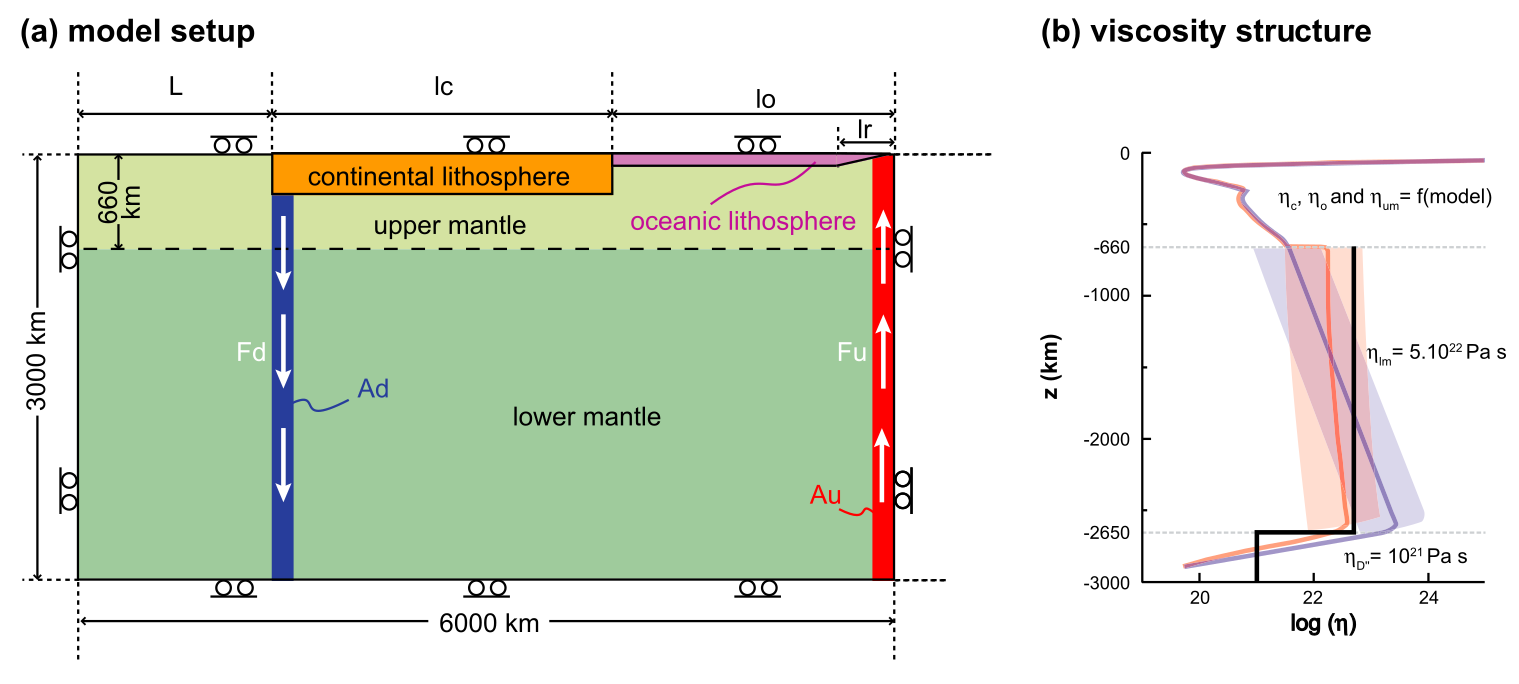
\includegraphics[width=15cm]{python_codes/fieldstone_143/images/yahb13_a}\\
{\captionfont 
Taken from \cite{yahb13}. Initial configuration of the model. 
(a) Model setup. $L$: length of mantle space between the left-hand 
side of the box and the continental lithosphere; $l_c$ : length of continental lithosphere; 
$l_o$: length of oceanic lithosphere; 
$l_r=500~\si{\km}$: length corresponding to the thinning of the lithosphere due to the ridge; 
$F_d$: downwelling force; 
$F_u$: upwelling force. These buoyancy forces are implemented by setting variable
densities in the red and blue columns. The area of the columns is $A_d$ and $A_u$ for the downwelling and the
upwelling force, respectively. (b) Viscosity structure. $\eta_c$, $\eta_o$, and $\eta_{um}$ correspond
to the viscosity of the continental lithosphere, oceanic lithosphere, and upper mantle, respectively. The
viscosity of the lower mantle corresponds to a simplified profile (black line). The viscosity models from
\cite{civs12} (2012) are also provided (Family-A model in red and Family-B model in blue) as references. }
\end{center}

Please read the original paper for a justification of the chosen values for most 
of the parameters.

``The oceanic lithosphere is not attached
to the right-hand side of the box, for one upper mantle cell
separates it from the model box edge. This ensures that the
lithosphere is free to move laterally and is not affected by
the free-slip boundary condition imposed at the right side [...].''

``We [...] fixed typical thicknesses to
$200~\si{\km}$ and $100~\si{\km}$ [...] for the continental and the oceanic lithosphere, 
respectively. The width of the continental lithosphere is similarly
set in all our models to $2000~\si{\km}$.''

The density is set to $\rho_{ref}=3250~\si{\kg\per\cubic\meter}$ everywhere in the model box. Density
differences are only assigned to the upwelling and the
downwelling zones that drive, by buoyancy, the convection
cell. The density value in the upwelling ($\rho_u$) and
in the downwelling ($\rho_d$) areas depends on the buoyancy force
applied and are expressed as follows:
\begin{eqnarray}
\rho_u &=& \rho_{ref} - \frac{F_u}{\rho_{ref} g A_u} \\
\rho_d &=& \rho_{ref} + \frac{F_d}{\rho_{ref} g A_d} 
\end{eqnarray}
where $F_u$ and $F_d$ correspond to the absolute values of the 
upwelling and downwelling forces, respectively, and g is the gravitational 
acceleration set to $9.81~\si{\meter\per\square\second}$.
Note that the values for $A_u$ and $A_d$ is never specified!
Looking closely at Fig 6, we find that the blue and red zones are as wide as 
the thickness of the oceanic lithosphere, i.e. 100km.

These formula provide us with a learning opportunity:
If one fills the values for $F_u$, $\rho_{ref}$, $g$ and $A_u$ or $A_d$
in the formula we find {\it very} small density variations, i.e.
$\rho_u=3249.99895449$ and $\rho_d=3250.00104551$. 
These values are suspicious, and given the rather realistic viscosity
values and dimensions of the setup this is not likely to yield 
plausible velocities or strain rates. 

Looking closely, the nominator and denominator have the same dimensions, 
so that the ratio is dimensionless and can therefore not be 
added or subtracted to a density! Upon my contacting the authors they confirmed
my suspicion: the density term in the denominator is wrong.
The correct formula then read:
\begin{eqnarray}
\rho_u &=& \rho_{ref} - \frac{F_u}{ g A_u} \simeq 3246.60211~\si{\kg\per\cubic\meter} \\
\rho_d &=& \rho_{ref} + \frac{F_d}{ g A_d} \simeq 3253.64059~\si{\kg\per\cubic\meter} 
\end{eqnarray}

The viscosity in the lower mantle corresponds
to a very simplified profile: From $660~\si{\km}$ to $2650~\si{\km}$ depth,
the viscosity is set to $\eta_{lm}=5\cdot 10^{22}~\si{\pascal\second}$. 
Below, the viscosity is set to $10^{21}~\si{\pascal\second}$ (D'' layer). 

Above the lower mantle, the viscosities
are not well resolved and therefore need to be tested.
The authors ``considered the viscosity of the continental 
lithosphere, of the oceanic lithosphere, and of the
upper mantle as linear and constant.''

\begin{center}
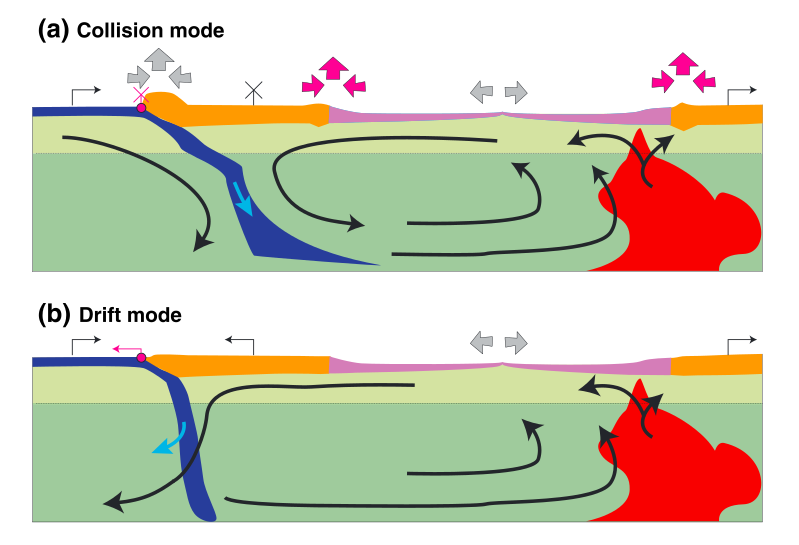
\includegraphics[width=12cm]{python_codes/fieldstone_143/images/yahb13_b}\\
{\captionfont 
Taken from \cite{yahb13}. 
Sketch of the mantle convective cell flow in (a) collision mode and (b) drift mode. In the
collision mode, the anchored slab does not retreat and prevents the trench-ward motion of the upper plate
and is thus blocked. In drift mode, the subducting slab is retreating and accommodates the oceanic litho-
sphere convergence that can freely move. Thick black and blue arrows show mantle flow and slab motion,
respectively. Thin black and magenta arrows correspond to the lithosphere and trench displacements,
respectively. These thin arrows are replaced by crosses when the motion is zero with respect to the upwelling.
Large grey and magenta arrows correspond to compressional and extensional areas at active and passive plate
margins, respectively.
}
\end{center}

%%%%%%%%%%%%%%%%%%%%%%%%%%%%%%%%%%%%%%%%%%%%%%%%%%%%%%%%%%%%%%%%%%%%%%%%%%%%%%%%%%%%%%%
\section*{About the code}

The code relies on the Finite Element method to solve the mass and momentum conservation
equations for an isothermal incompressible fluid. 
Quadrilateral elements are used and the stable $Q_2\times Q_1$ pair is used.
Note that in the light of the first round of results I have also implemented
the $Q_2\times P_{-1}$ pair (unless mentioned the first element is used). 
Since free slip boundary conditions are used on all sides there is a pressure 
nullspace which is removed by requiring that $\int_\Omega p \; dV=0$.
Note that this code is rather inefficient and that although resolutions above $300 \times 150$ 
are attainable, the required cpu time makes them undesirable\footnote{On my laptop
a 400x200 mesh yields a matrix that is built in approx. 1000s! and memory requirements 
seem to be above 10Gb.}. 

\newpage
%%%%%%%%%%%%%%%%%%%%%%%%%%%%%%%%%%%%%%%%%%%%%%%%%%%%%%%%%%%%%%%%%%%%%%%%%%%%%%%%%%%%%%%
\section*{Collision mode}

This corresponds to paragraph 19 and after in the paper. 

In the collision mode, $L = 0$ and the lithosphere cannot
move freely above the convection cell. The net driving force involved in this
example amounts to $2\cdot 10^{13}~\si{\newton\per\meter}$. This total force is evenly
distributed ($F_u = F_d = 10^{13}~\si{\newton\per\meter}$). 


\begin{center}
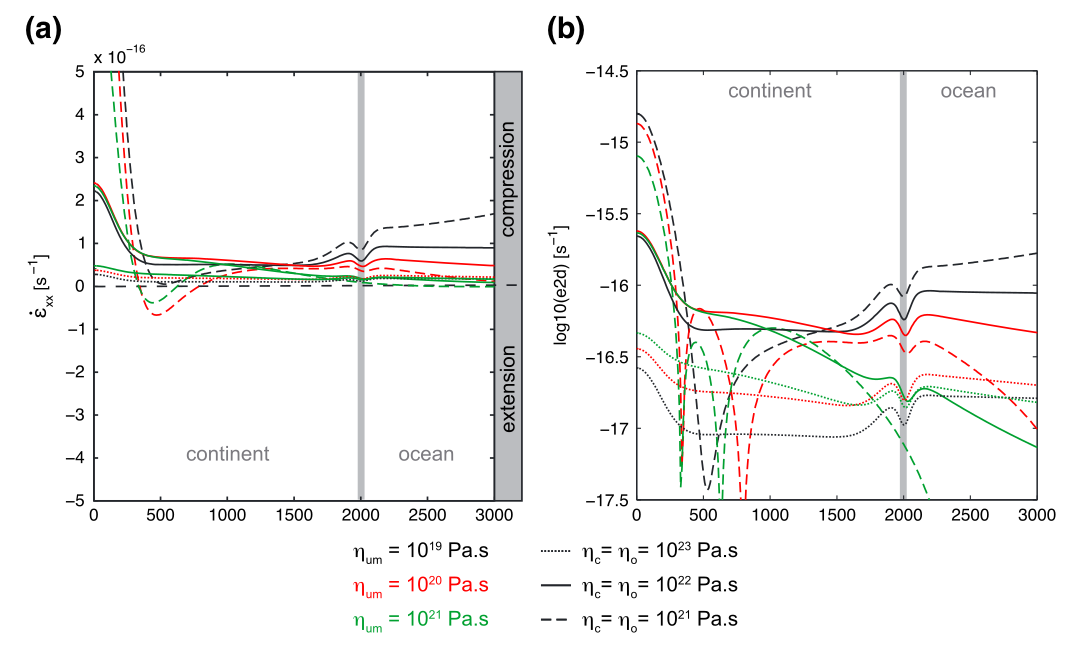
\includegraphics[width=14cm]{python_codes/fieldstone_143/images/fig4}\\
{\captionfont (a) Shortening rate  $\dot{\varepsilon}_{xx}$ 
(horizontal component of the strain rate tensor) at the surface across the
3000 km long continental and oceanic lithospheres ($L = 0~\si{\km}$, 
$l_c = 2000~\si{\km}$, $F_d = F_u = 10^{13}~\si{\newton\per\meter}$. 
Positive values of  $\dot{\varepsilon}_{xx}$ correspond to compression\footnote{Their convention
is then opposite of mine so I plot the negative of my measurements to match theirs.}. 
(b) Logarithm of the second invariant of the strain rate (e2d) along the same profile.}
\end{center}

\begin{center}
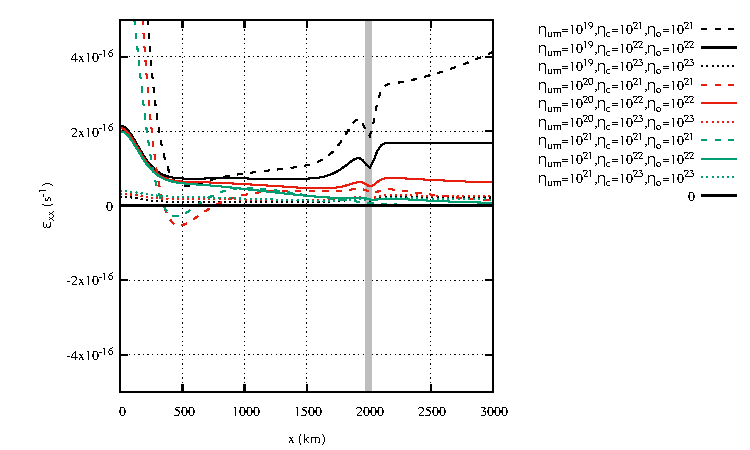
\includegraphics[width=8.6cm]{python_codes/fieldstone_143/results/fig4/fig4a}
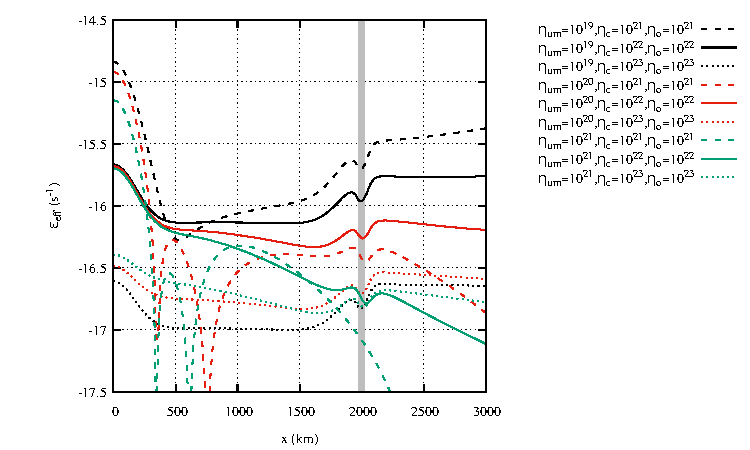
\includegraphics[width=8.6cm]{python_codes/fieldstone_143/results/fig4/fig4b}\\
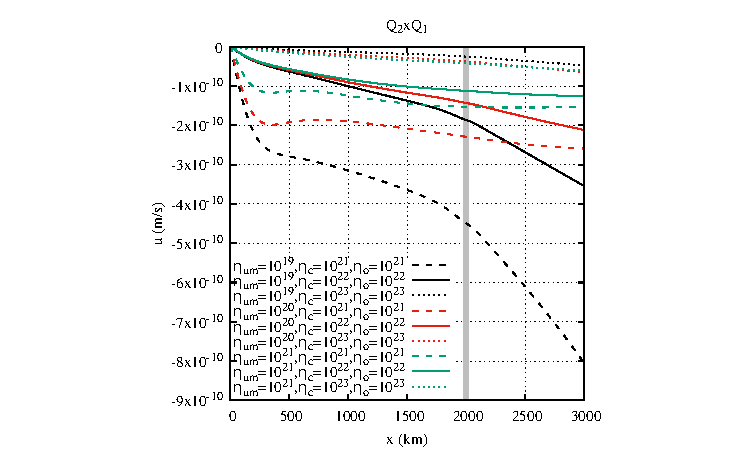
\includegraphics[width=8.6cm]{python_codes/fieldstone_143/results/fig4/fig4_u}
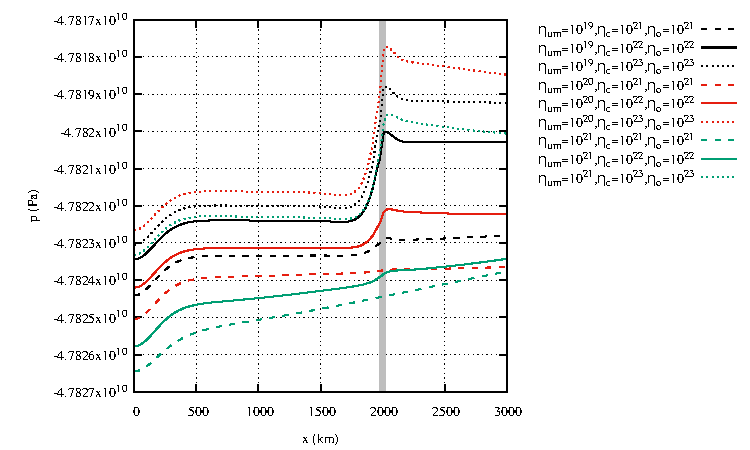
\includegraphics[width=8.6cm]{python_codes/fieldstone_143/results/fig4/fig4_p}\\
{\captionfont Data obtained with {\tt script\_fig4} with resolution $200\times 100$.
Replication is possible and aside from 19/21/21 all curves agree.}
\end{center}

If we now run the same models using the discontinuous pressure element, we
observe substantial differences in the results:

\begin{center}
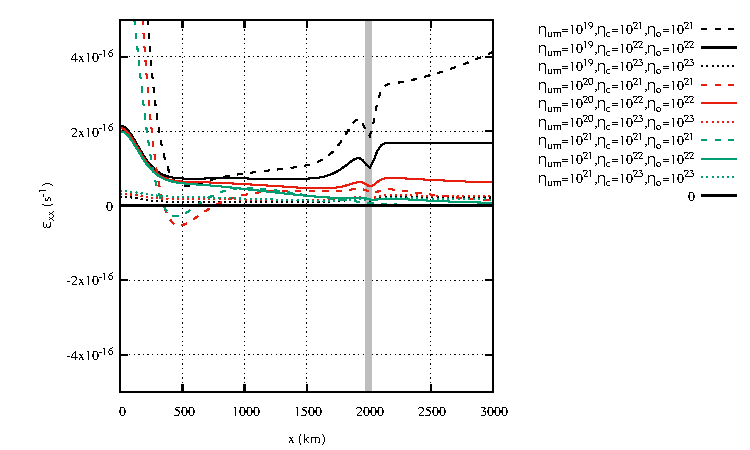
\includegraphics[width=8.6cm]{python_codes/fieldstone_143/results/fig4/fig4a}
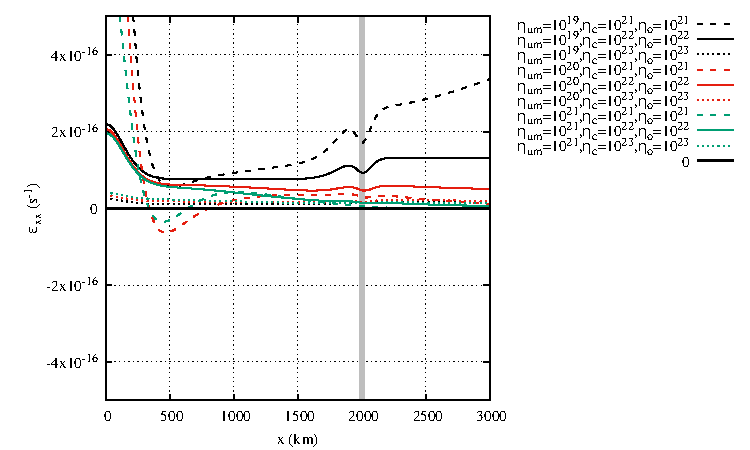
\includegraphics[width=8.6cm]{python_codes/fieldstone_143/results/fig4_q2pm1/fig4a}\\
{\captionfont  Left: $Q_2\times Q_1$; Right: $Q_2\times P_{-1}$. Both at resolution $200\times 100$.}
\end{center}

 

\begin{center}
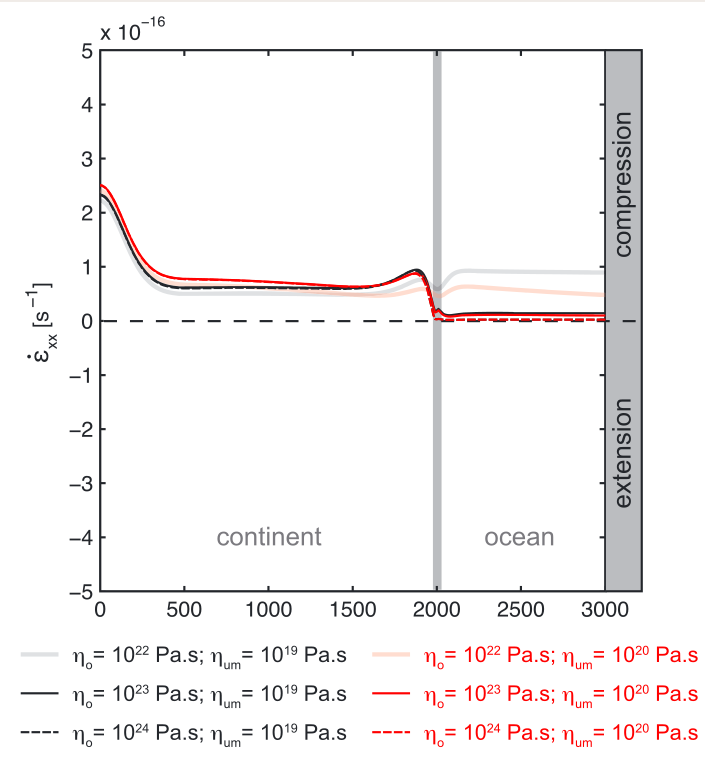
\includegraphics[width=4cm]{python_codes/fieldstone_143/images/fig5}
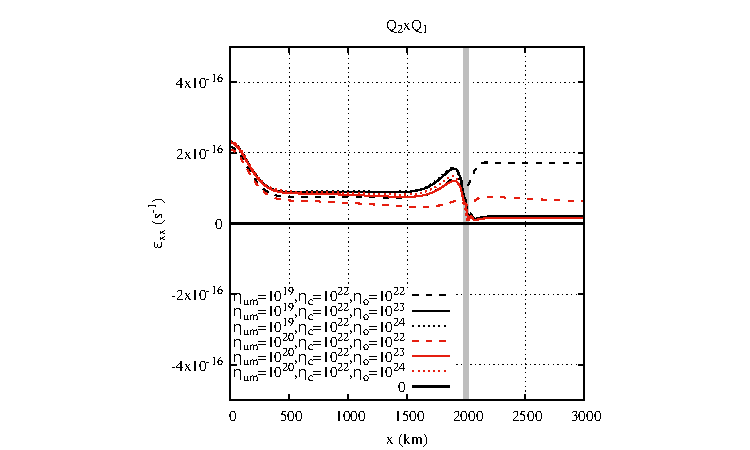
\includegraphics[width=6.5cm]{python_codes/fieldstone_143/results/fig5/fig5a}
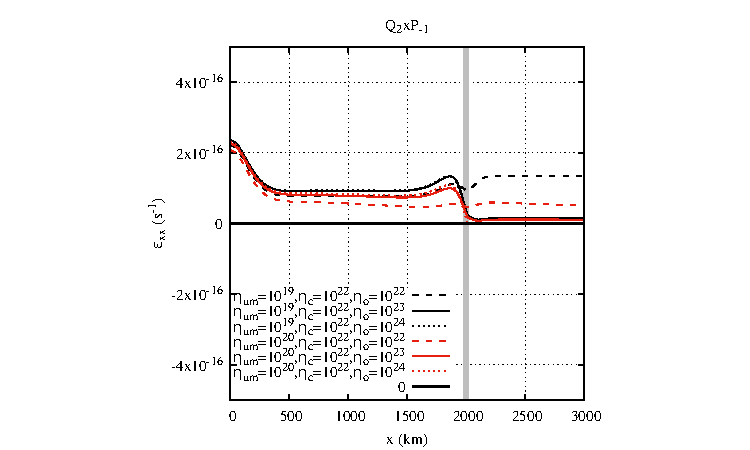
\includegraphics[width=6.5cm]{python_codes/fieldstone_143/results/fig5_q2pm1/fig5a}\\
{\captionfont Horizontal component of the strain rate $\dot{\varepsilon}_{xx}$
across the 3000 km long continental and oceanic lithospheres
($L = 0~\si{\km}$ and $l_c = 2000~\si{\km}$), for a variety of
oceanic $\eta_o$ and upper mantle $\eta_um$ viscosities. The viscosity
of the continental lithosphere $\eta_c$ is set to $10^{22}~\si{\pascal\second}$.
Left: fig 5 from the paper. Middle: obtained with this  {\tt script\_fig5},
$Q_2\times Q_1$; Right: same with $Q_2\times P_{-1}$.}
\end{center}

\begin{center}
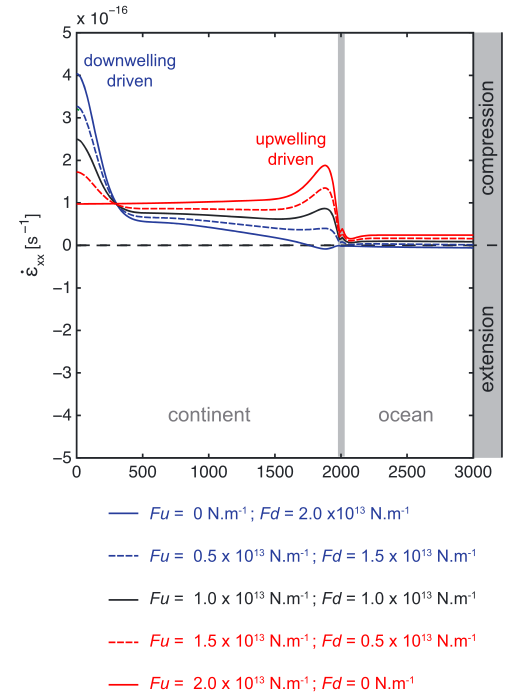
\includegraphics[width=7cm]{python_codes/fieldstone_143/images/fig6}
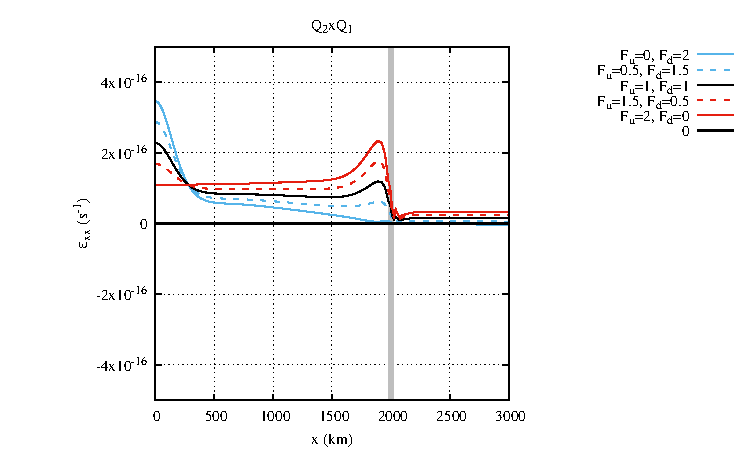
\includegraphics[width=10.5cm]{python_codes/fieldstone_143/results/fig6/fig6a}\\
{\captionfont 
Strain rate at the surface across the $3000~\si{\km}$ long continental and 
oceanic lithospheres ($L=0~\si{\km}$ and $l_ c=2000~\si{\km}$).
Reference model, $\eta_{um}=10^{20}~\si{\pascal\second}$, 
$\eta_c=10^{22}~\si{\pascal\second}$, $\eta_o=10^{23}~\si{\pascal\second}$. 
Left: Fig 6 from \cite{yahb13}, Right: obtained with this  {\tt script\_fig6}.}
\end{center}

%---------------------------------------------------
\subsubsection*{Testing influence of resolution}

Results are not fundamentally different between the two types of elements.
\begin{center}
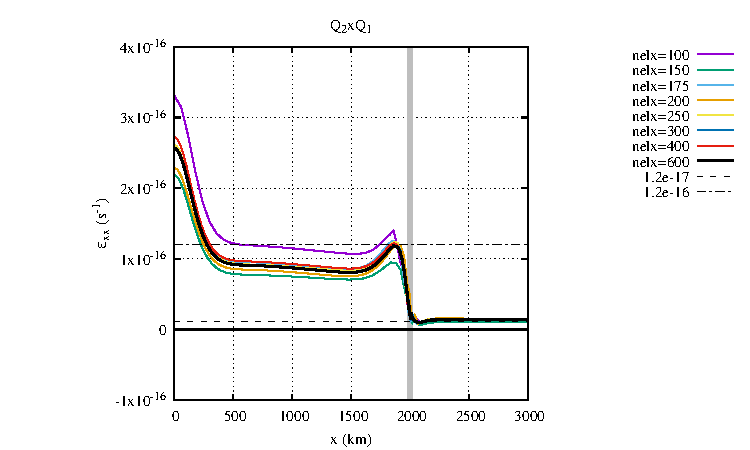
\includegraphics[width=7.5cm]{python_codes/fieldstone_143/results/resolutions/fig_resolutions}
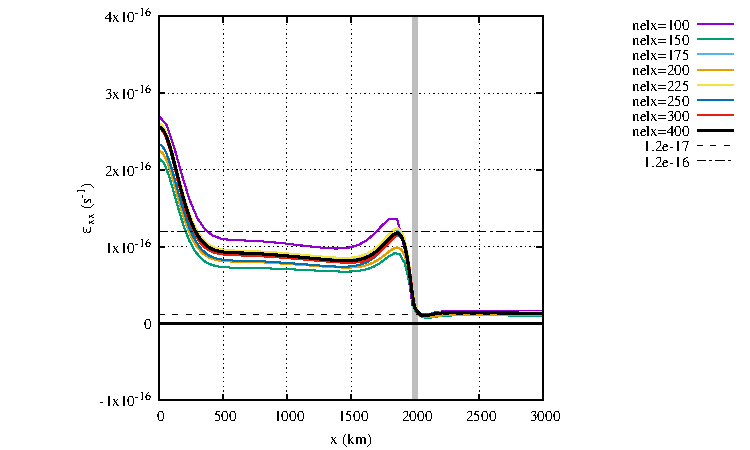
\includegraphics[width=7.5cm]{python_codes/fieldstone_143/results/resolutions_q2pm1/fig_resolutions}\\
{\captionfont 
Reference model, $\eta_{um}=10^{20}~\si{\pascal\second}$, 
$\eta_c=10^{22}~\si{\pascal\second}$, $\eta_o=10^{23}~\si{\pascal\second}$. 
Obtained with this  {\tt script\_resolutions}.
Left: $Q_2\times Q_1$; Right: $Q_2\times P_{-1}$.}
\end{center}

\newpage

\begin{center}
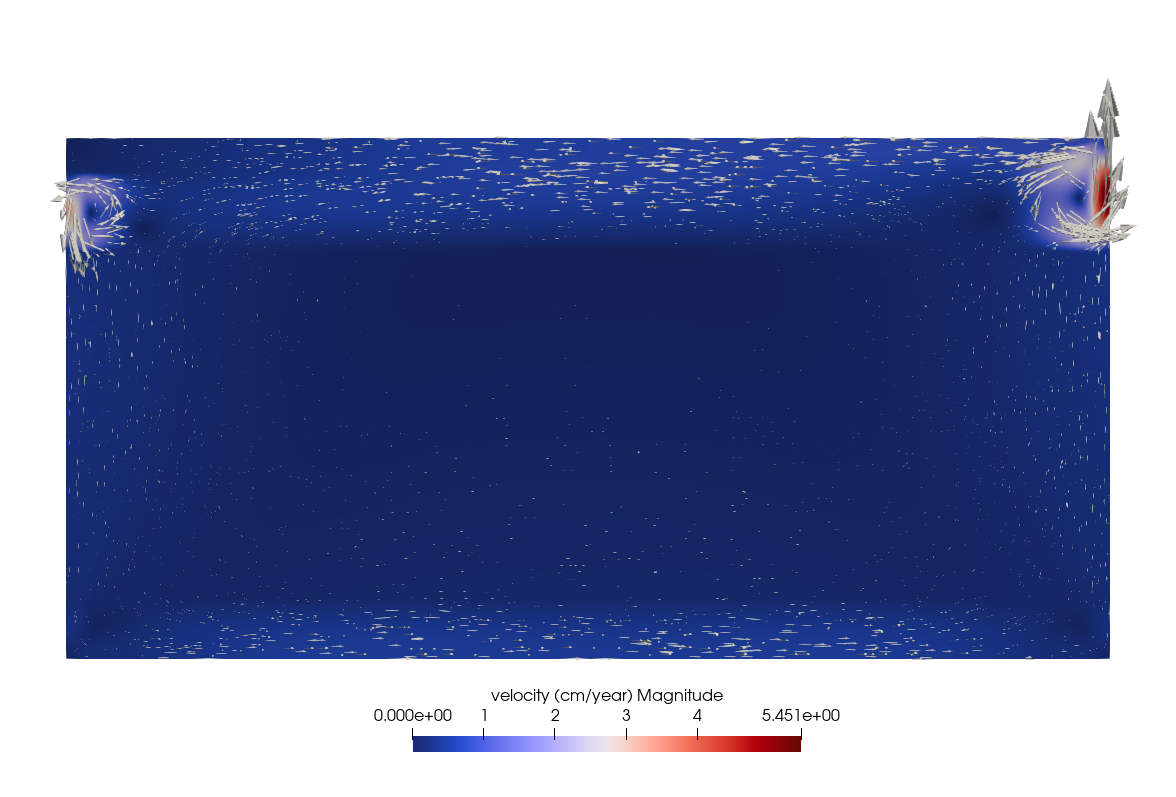
\includegraphics[width=8cm]{python_codes/fieldstone_143/results/resolutions/vel}
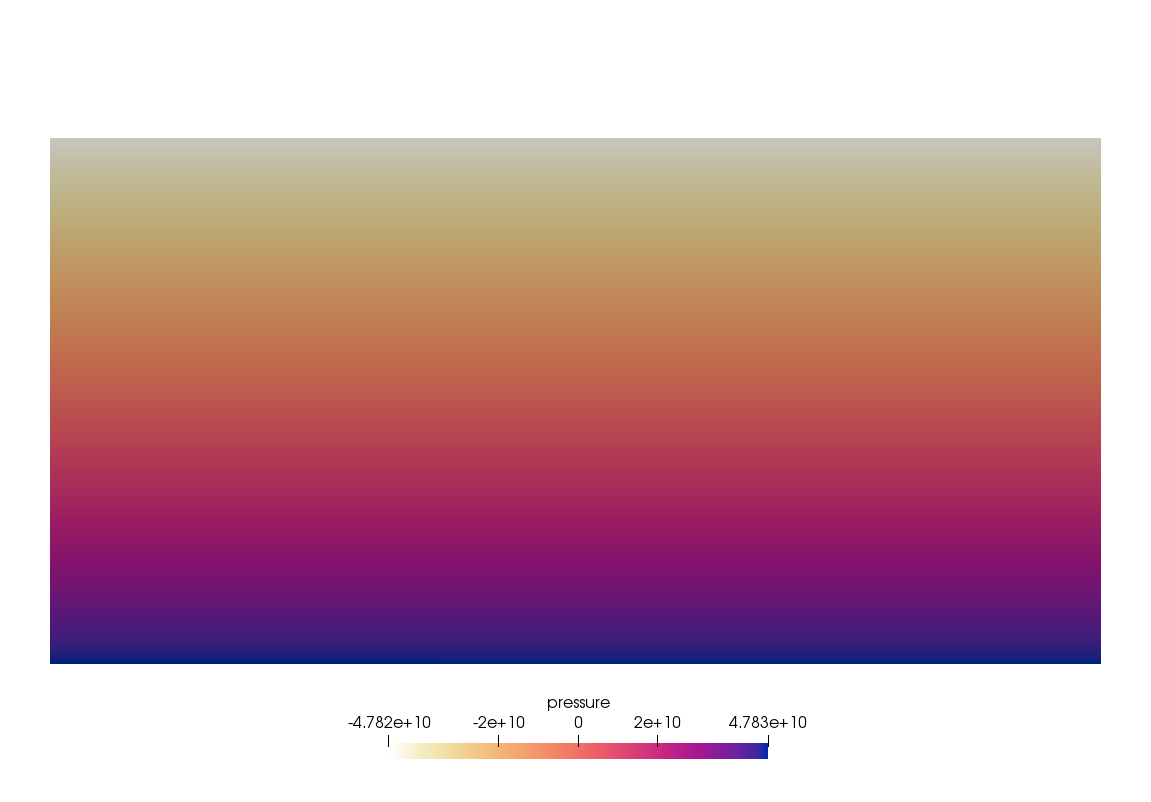
\includegraphics[width=8cm]{python_codes/fieldstone_143/results/resolutions/press}\\
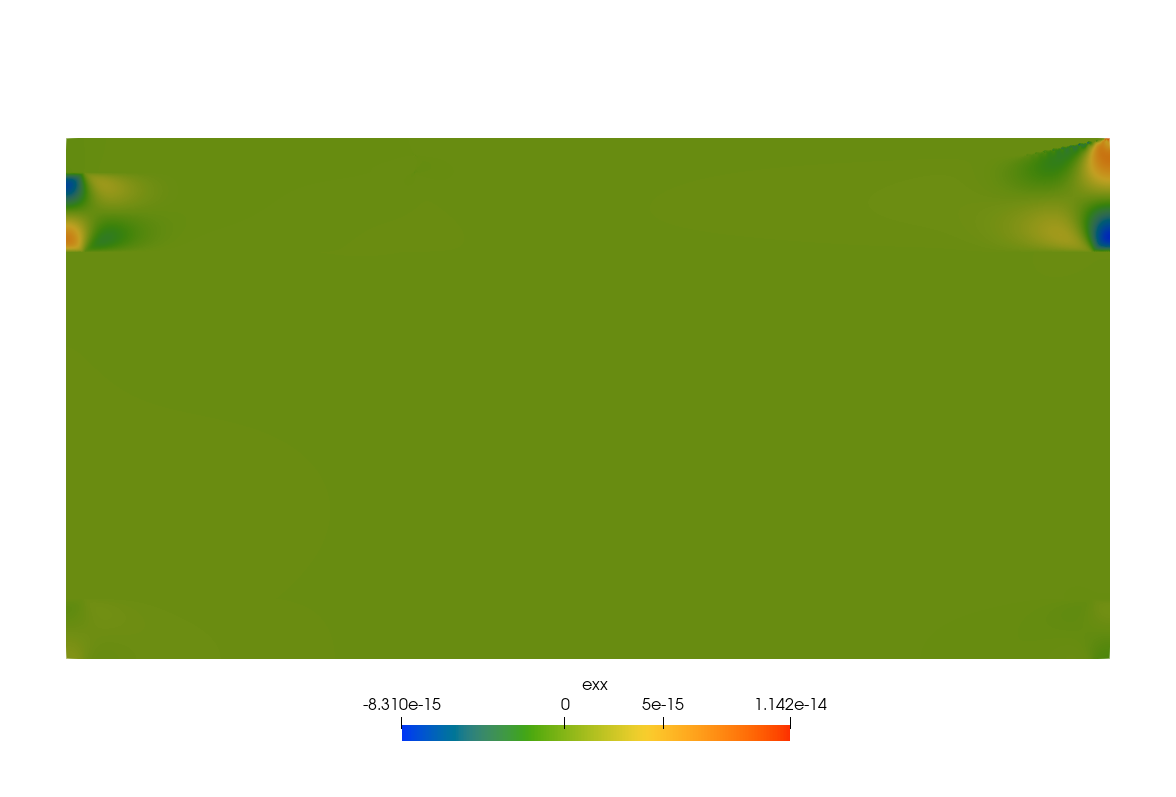
\includegraphics[width=8cm]{python_codes/fieldstone_143/results/resolutions/exx}
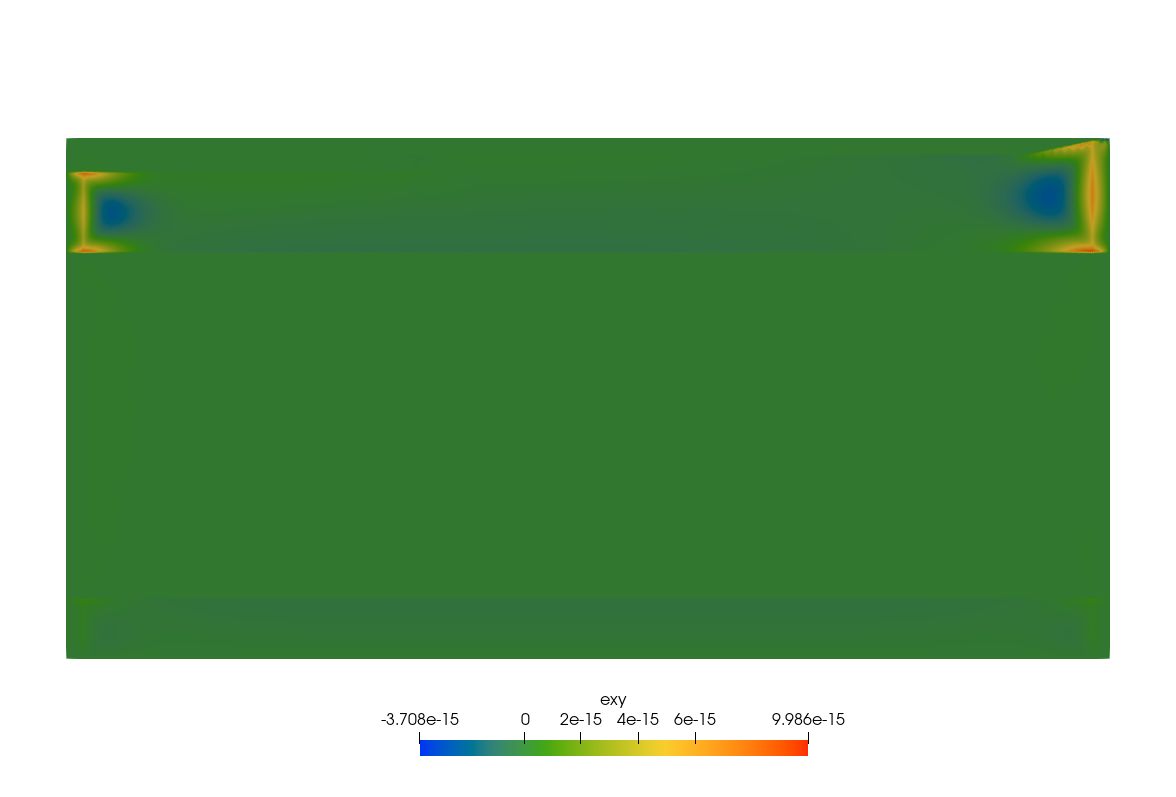
\includegraphics[width=8cm]{python_codes/fieldstone_143/results/resolutions/exy}\\
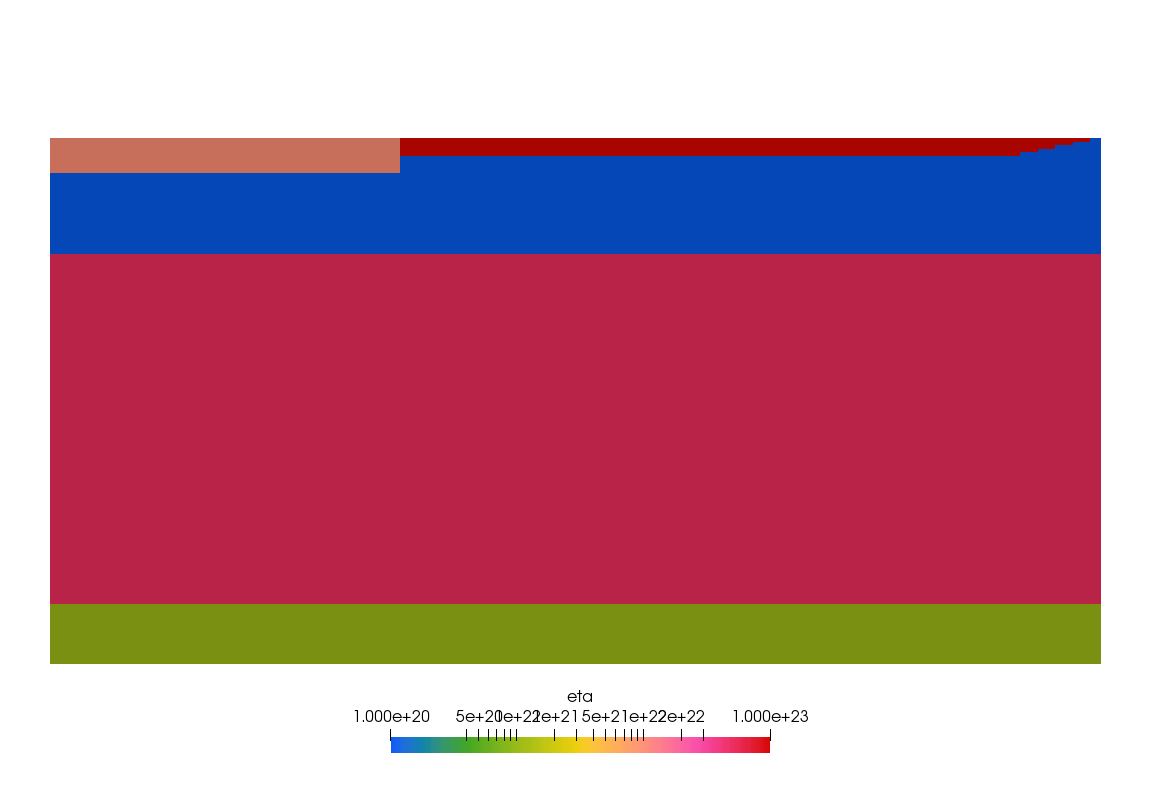
\includegraphics[width=8cm]{python_codes/fieldstone_143/results/resolutions/eta}
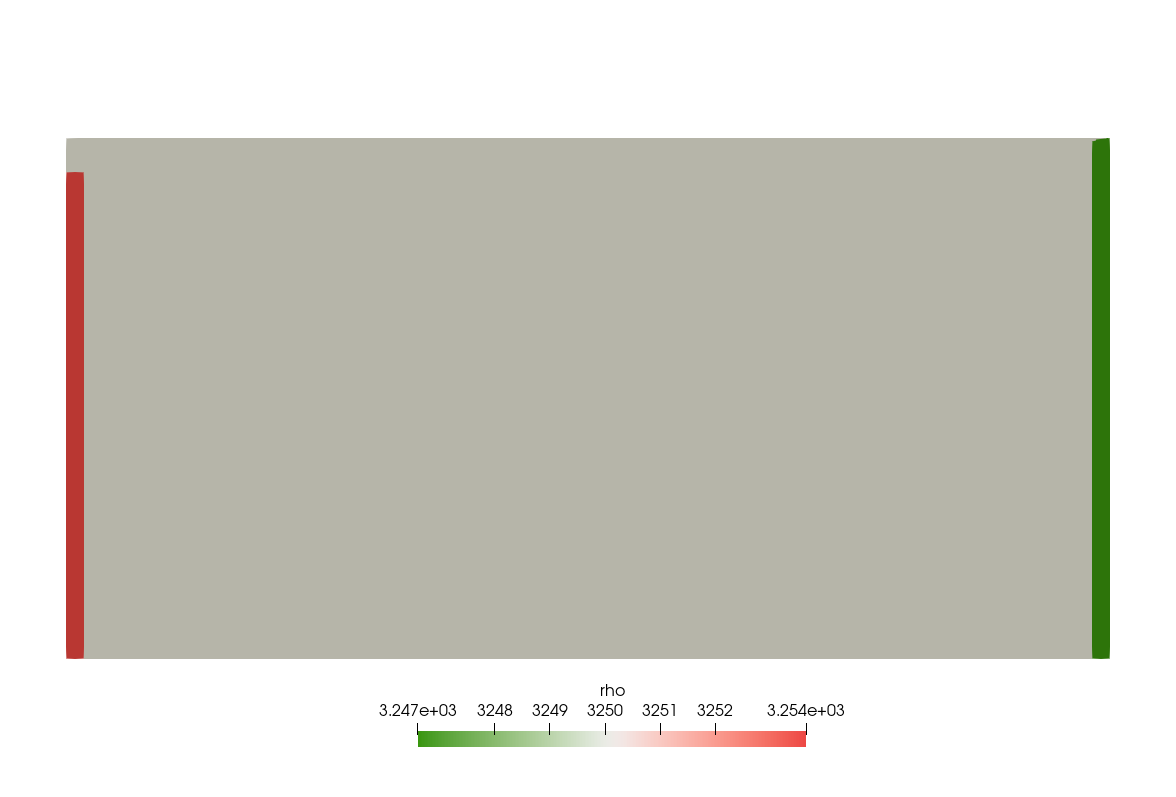
\includegraphics[width=8cm]{python_codes/fieldstone_143/results/resolutions/rho}\\
{\captionfont Reference model, nelx=300. Resolution is then 20 km while theirs is 10 km.}
\end{center}


%---------------------------------------------------
\subsubsection*{Testing the influence of width of areas}

In the paper the exact width of the high/low density zones is not specified. 
Based on the figures we have assumed that there were 100~\si{\km} wide,
so it is time to explore this parameter.
\begin{center}
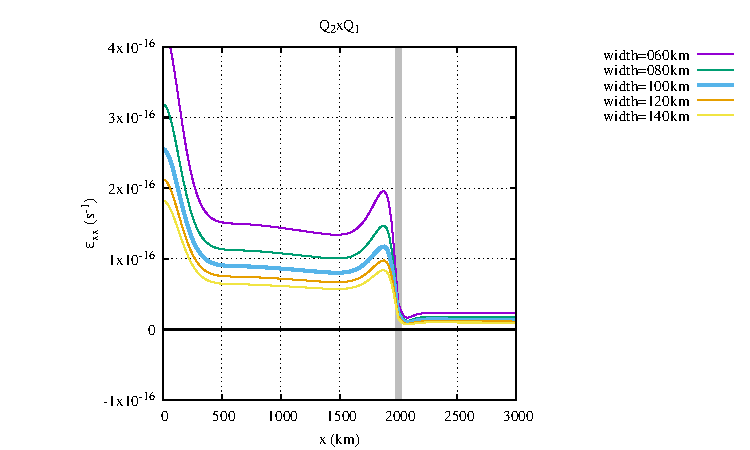
\includegraphics[width=8cm]{python_codes/fieldstone_143/results/widths_q2pm1/fig_widths}\\
{\captionfont Obtained with {\tt script\_widths} with $Q_2\times P_{-1}$ elements. Resolution 300x150, h=20km.}
\end{center}



\newpage
%%%%%%%%%%%%%%%%%%%%%%%%%%%%%%%%%%%%%%%%%%%%%%%%%%%%%%%%%%%%%%%%%%%%%%%%%%%%%%%%%%%%%%%
\section*{Drift versus collision mode}

In this case we explore $L=0,1000,3000~\si{\km}$, see paper for geodynamical 
implications. Also I have not bothered to carry out the measurements of their fig 8.

\begin{center}
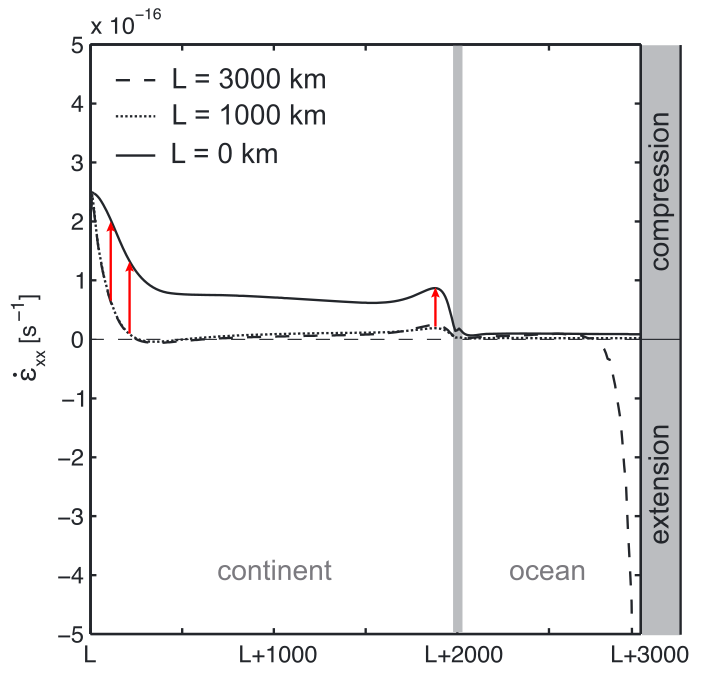
\includegraphics[width=7cm]{python_codes/fieldstone_143/images/fig9}
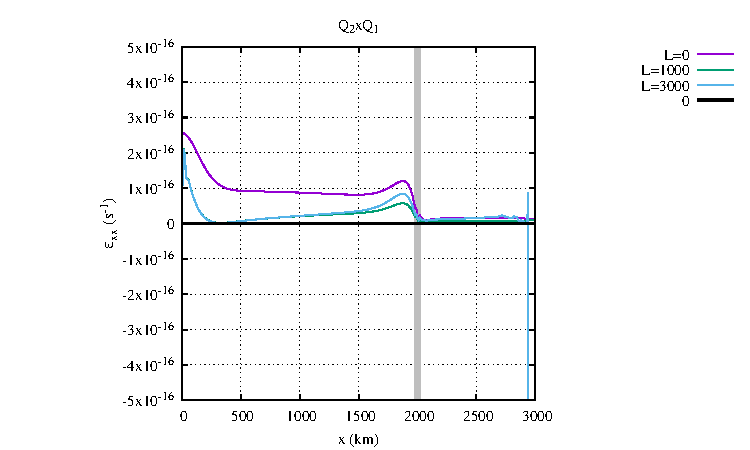
\includegraphics[width=10cm]{python_codes/fieldstone_143/results/fig9/fig9}\\
{\captionfont Horizontal component of the strain rate $\dot{\varepsilon}_{xx}$ at
the surface across the 3000 km long continental and oceanic
lithospheres. Red arrows show the jump that occurs at the
transition from drift mode to collision mode.
Left: fig 9 of the paper. Right: obtained with this stone.}
\end{center}



\begin{center}
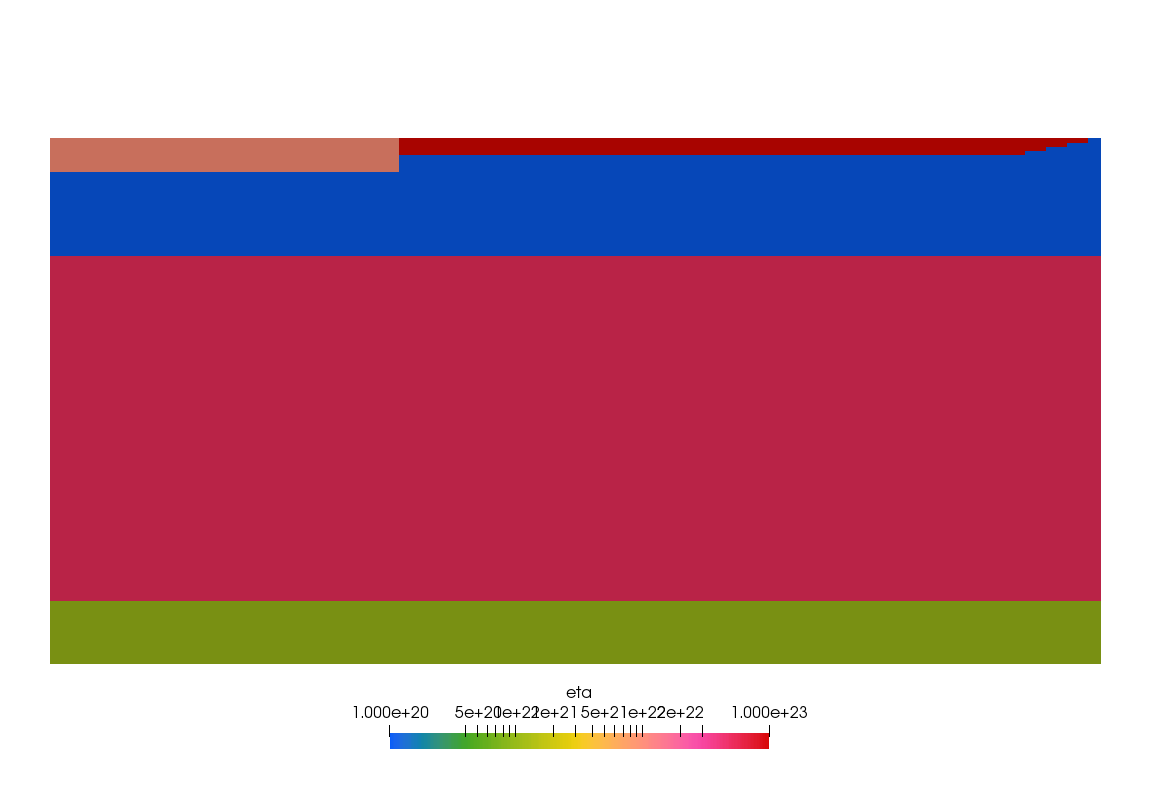
\includegraphics[width=5.7cm]{python_codes/fieldstone_143/results/fig9/eta0000}
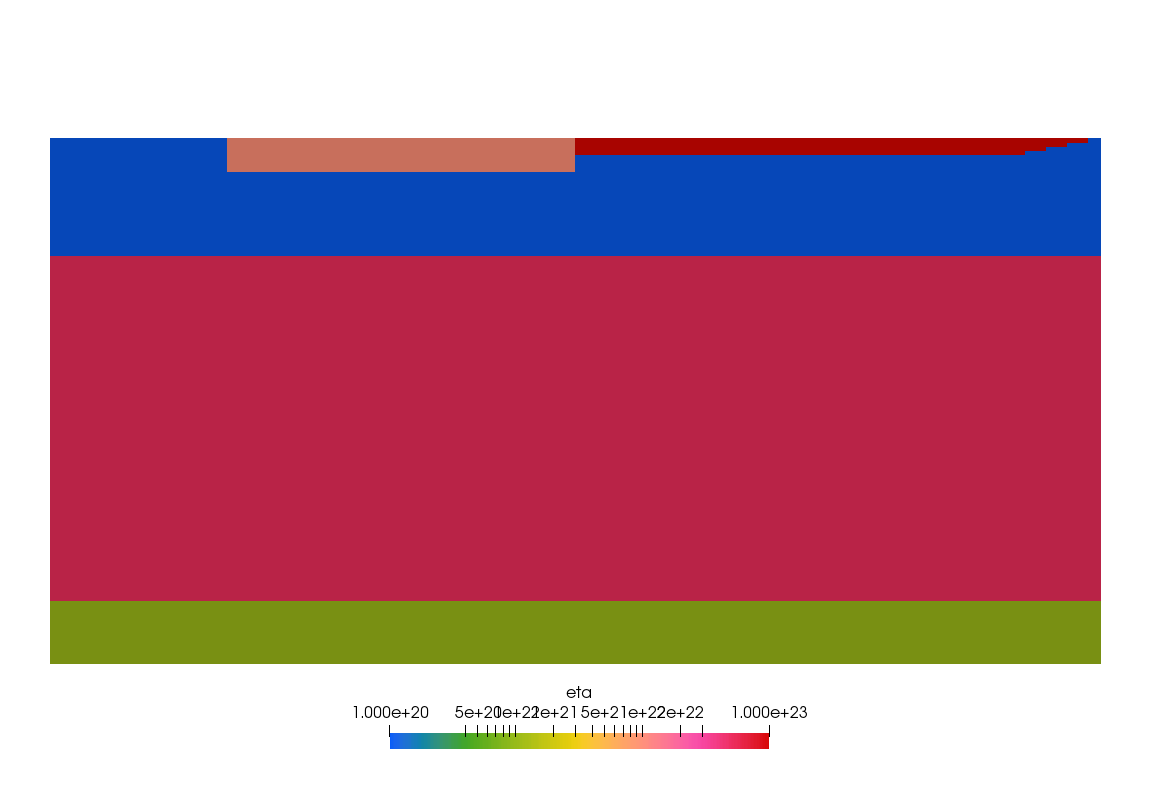
\includegraphics[width=5.7cm]{python_codes/fieldstone_143/results/fig9/eta1000}
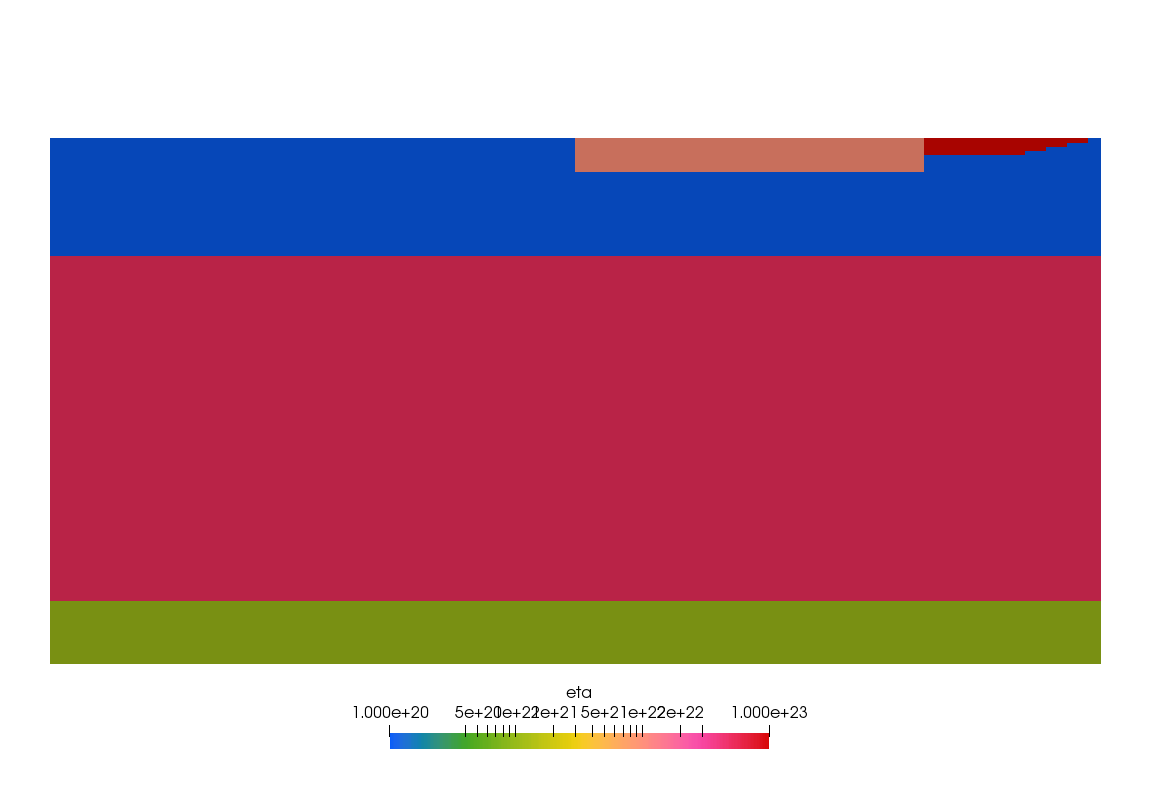
\includegraphics[width=5.7cm]{python_codes/fieldstone_143/results/fig9/eta3000}\\
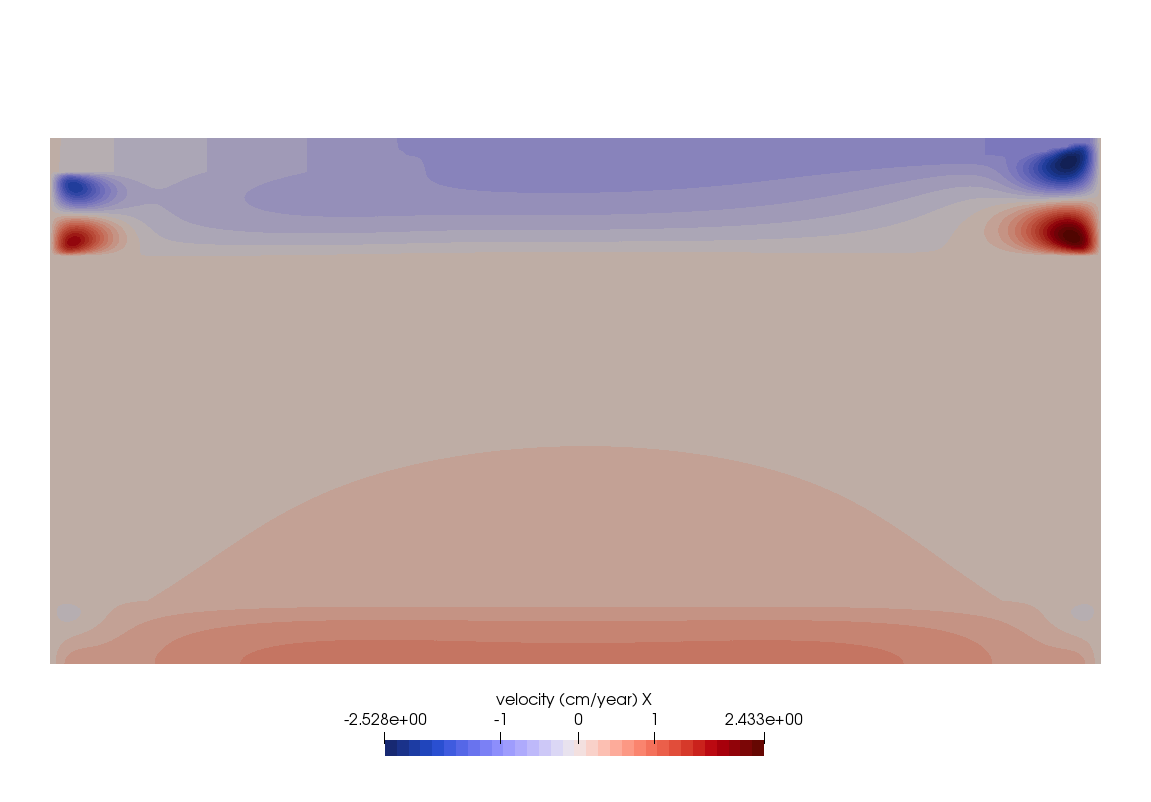
\includegraphics[width=5.7cm]{python_codes/fieldstone_143/results/fig9/u0000}
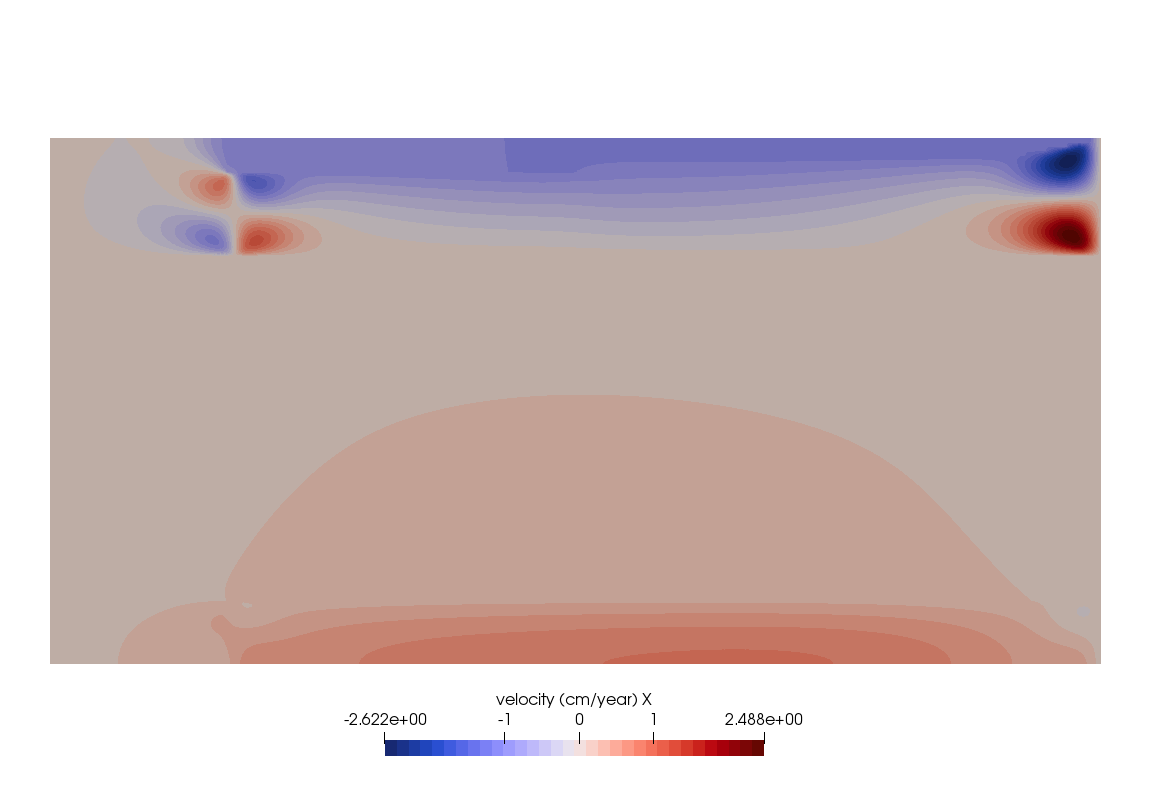
\includegraphics[width=5.7cm]{python_codes/fieldstone_143/results/fig9/u1000}
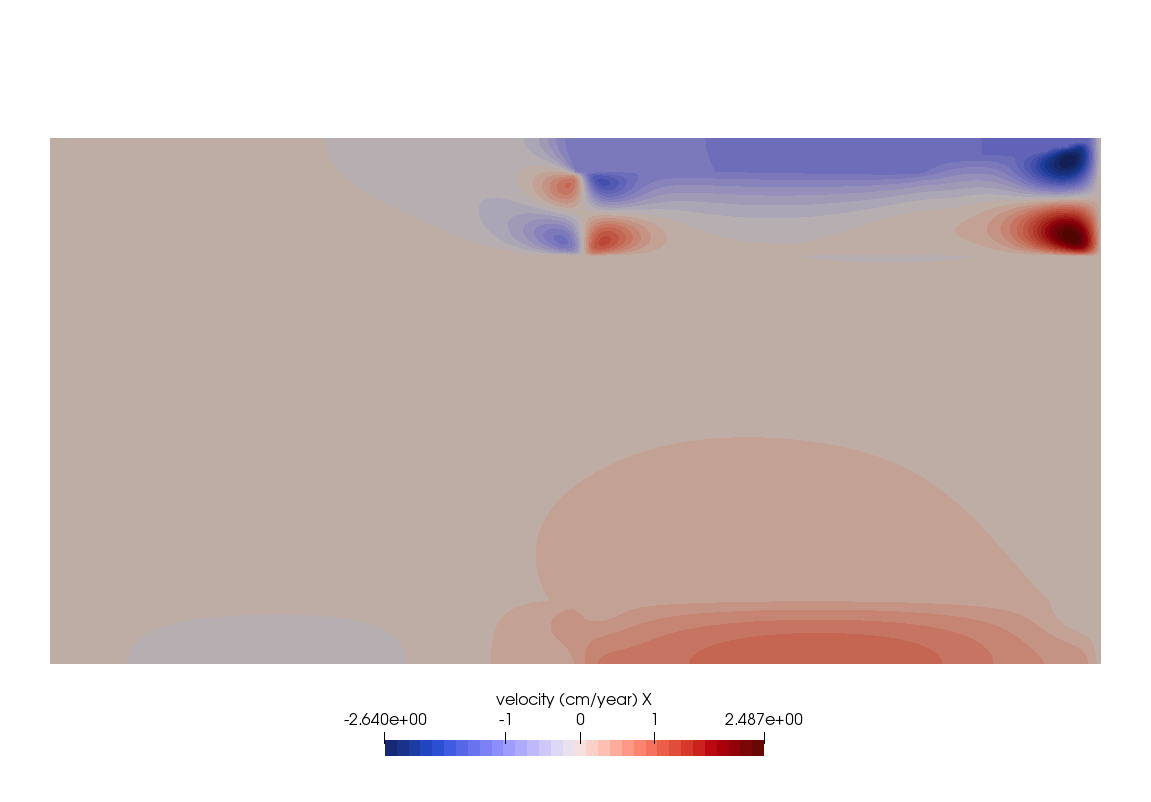
\includegraphics[width=5.7cm]{python_codes/fieldstone_143/results/fig9/u3000}\\
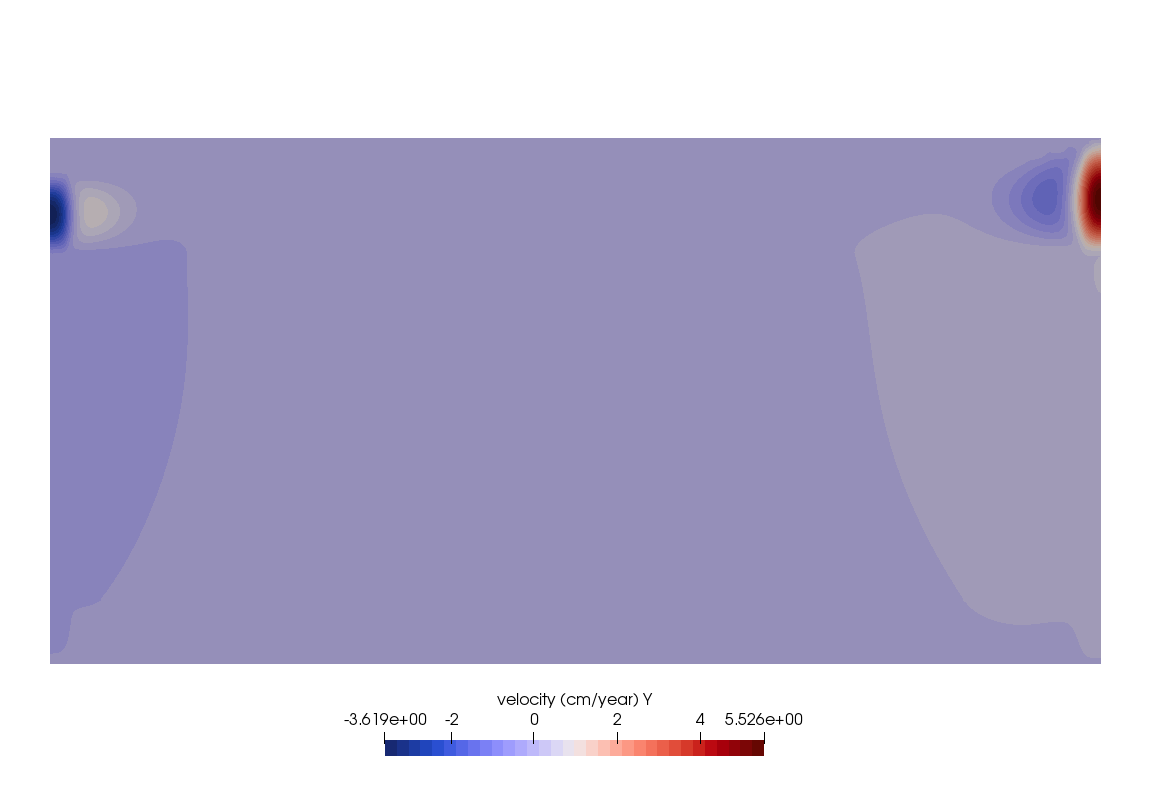
\includegraphics[width=5.7cm]{python_codes/fieldstone_143/results/fig9/v0000}
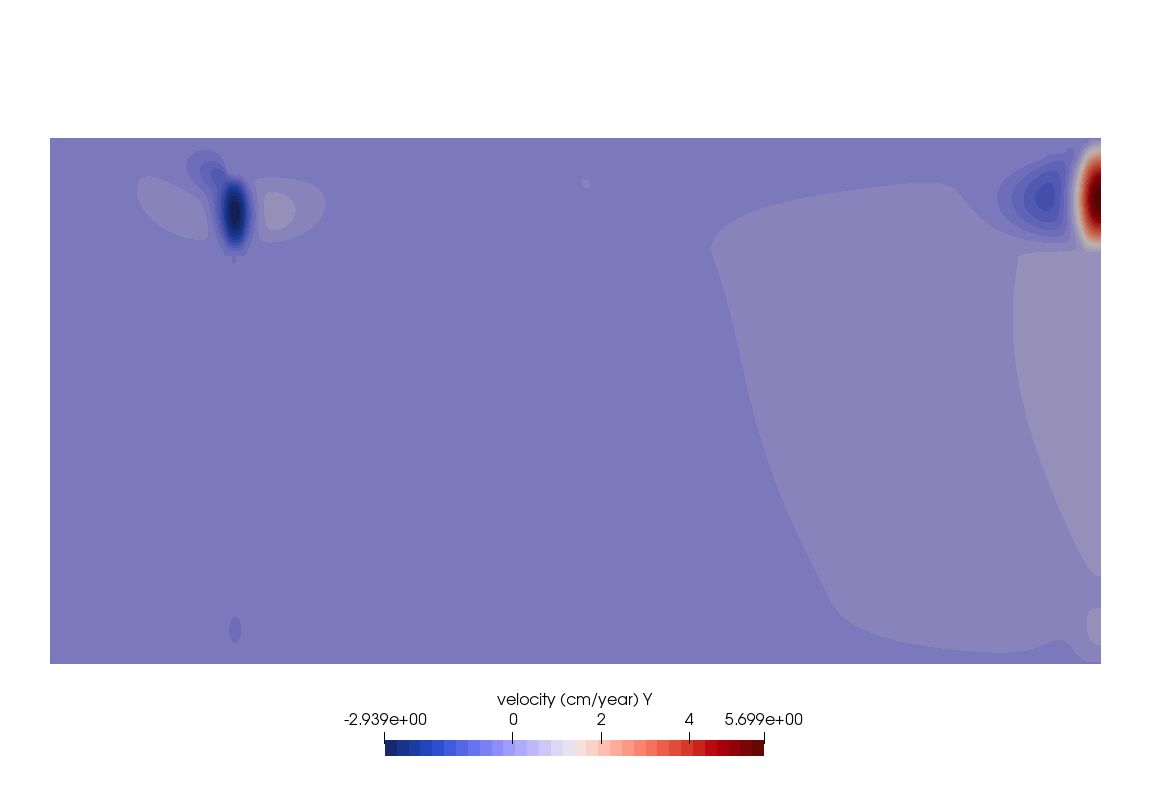
\includegraphics[width=5.7cm]{python_codes/fieldstone_143/results/fig9/v1000}
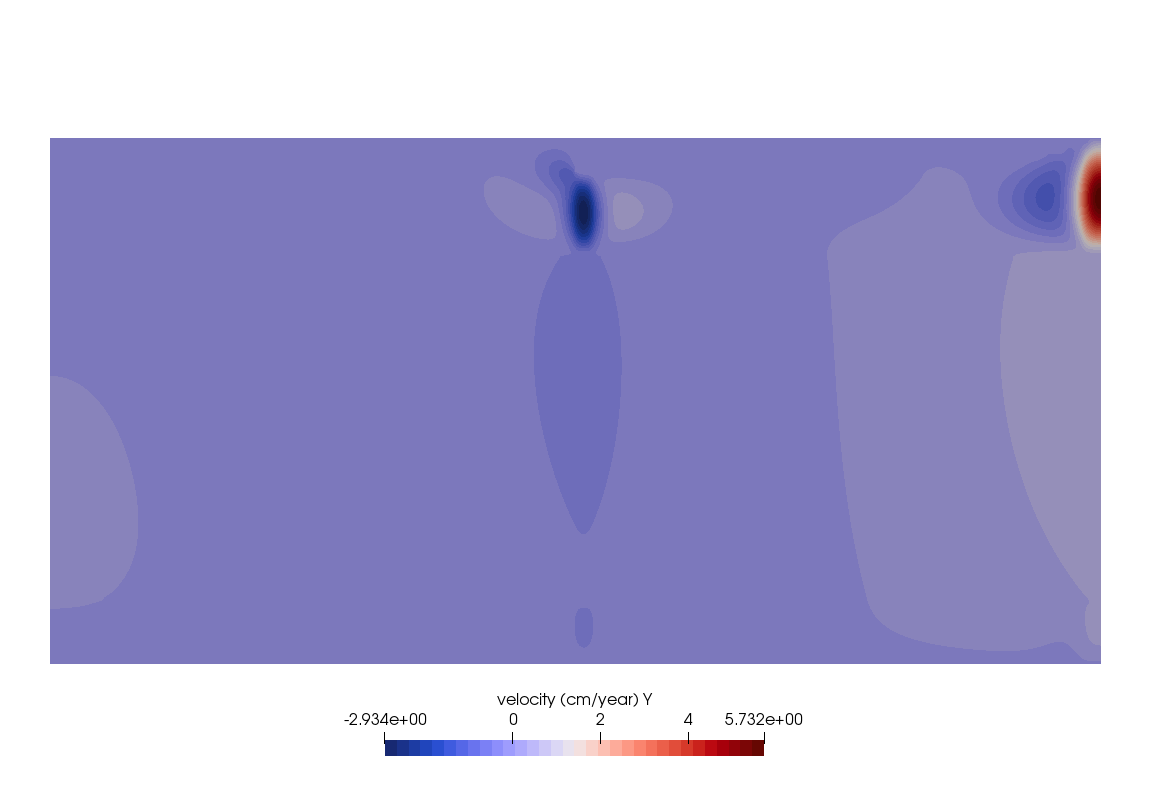
\includegraphics[width=5.7cm]{python_codes/fieldstone_143/results/fig9/v3000}\\
{\captionfont From left to right: L=0km, L=10000km, L=3000km.}
\end{center}

----------------------------------------------------------------

ToDo:

- implement Q2P-1

- redo figure 8 of paper

- make code faster?

































